% Este trabalho está licenciado sob a Licença Atribuição-CompartilhaIgual 4.0 Internacional Creative Commons. Para visualizar uma cópia desta licença, visite http://creativecommons.org/licenses/by-sa/4.0/deed.pt_BR ou mande uma carta para Creative Commons, PO Box 1866, Mountain View, CA 94042, USA.

\chapter{Funções}\label{cap_fun}
\thispagestyle{fancy}

Uma \hl{\emph{função} (ou método) é um \emph{subprograma} (ou subalgoritmo)}, um bloco de programação para o processamento de uma tarefa e que pode ser chamado à execução, sempre que necessário, pelo programa a que pertence.

\section{Funções Predefinidas e Módulos}\label{cap_fun_sec_buildin}

\subsection{Funções Predefinidas}

Como o nome indica, \hl{\emph{funções predefinidas} são aquelas disponíveis por padrão na linguagem de programação}, i.e. sem a necessidade de serem explicitamente definidas no código. As \hl{funções predefinidas do {\python}} podem ser consultadas em
\begin{center}
  \url{https://docs.python.org/3/library/functions.html}
\end{center}

Nós já vinhamos utilizando várias dessas funções.

\subsubsection{Entrada e Saída de Dados}

Na entrada e saída de dados, utilizamos
\begin{itemize}
\item \hl{{\lstinline+input()+}}

  Essa função lê uma linha digitada no \textit{prompt}, converte-a em uma \textit{string} e a retorna. Admite como entrada uma \textit{string} que é impressa no \textit{prompt} antes da leitura.

\item \hl{{\lstinline+print()+}}

  Essa função recebe um objeto e o imprime em formato texto, por padrão, no \textit{prompt} de saída.

\begin{lstlisting}
>>> s = input('Olá, qual o seu nome? ')
Olá, qual o seu nome? Fulane
>>> print(f'Bem vinde, {s}!')
Bem vinde, Fulane!
\end{lstlisting}
\end{itemize}

\subsubsection{Construtores de Dados}

Temos as funções que constroem objetos de classes de números:
\begin{itemize}

\item \hl{{\lstinline+bool()+}}

  Recebe um objeto e retorna outro da classe \lstinline+bool+.

\begin{lstlisting}
>>> bool(0)
False
>>> bool(1)
True
>>> bool('')
False
>>> bool('0')
True
\end{lstlisting}
  
\item \hl{{\lstinline+int()+}}

  Recebe um número ou \textit{string} \lstinline+x+ e retorna um objeto da classe \lstinline+int+.

\begin{lstlisting}
>>> int(-2.1)
-2
>>> int(3.9)
3
>>> int(5.5)
5
>>> int('51')
51
\end{lstlisting}

\item \hl{{\lstinline+float()+}}

  Recebe um número ou \textit{string} \lstinline+x+ e retorna um objeto da classe \lstinline+float+.

\begin{lstlisting}
>>> float(1)
1.0
>>> float('-2.7')
-2.7
\end{lstlisting}

\item \hl{{\lstinline+complex()+}}

  Recebe as partes real e imaginária de um número complexo ou uma \textit{string} e retorna um objeto da classe \lstinline+complex+.

\begin{lstlisting}
>>> complex(2,-3)
(2-3j)
>>> complex('-7+5j')
(-7+5j)
\end{lstlisting}
\end{itemize}

Para a construção de objetos de classes de coleção de dados, temos:
\begin{itemize}
\item \hl{{\lstinline+dict()+}}

  Recebe um mapeamento ou um iterável e retorna um objeto da classe \lstinline+dict+.

\item \hl{{\lstinline+list()+}}

  Recebe um iterável e retorna um objeto da classe \lstinline+list+.

\item \hl{{\lstinline+set()+}}

  Recebe um iterável e retorna um objeto da classe \lstinline+set+.

\item \hl{{\lstinline+str()+}}

  Recebe um objeto e retorna um outro da classe \lstinline+str+

\item \hl{{\lstinline+tuple+}}

  Recebe um iterável e retorna um objeto da classe \lstinline+tuple+.
\end{itemize}

Alguns construtores de iteráveis especiais são:
\begin{itemize}
\item \hl{{\lstinline+range()+}}

  Recebe até três inteiros \lstinline+start+, \lstinline+stop+, \lstinline+step+ e retorna um objeto iterável com início em \lstinline+start+ (incluído) e término em \lstinline+stop+ (excluído).

\begin{lstlisting}
>>> list(range(5))
[0, 1, 2, 3, 4]
>>> tuple(range(-10,1,2))
(-10, -8, -6, -4, -2, 0)
\end{lstlisting}

\item \hl{{\lstinline+enumerator()+}}

  Recebe um iterável e retorna um objeto \lstinline+enumerate+, um iterável de tuples que enumera os objetos do iterável de entrada.

\begin{lstlisting}
>>> cores = ['amarelo', 'azul', 'vermelho', ]
>>> list(enumerate(cores))
[(0, 'amarelo'), (1, 'azul'), (2, 'vermelho')]
\end{lstlisting}
\end{itemize}

\subsection{Módulos}

\hl{Módulos são bibliotecas computacionais}, i.e. um arquivo contendo funções (e/ou constantes) que podem ser incorporadas e usadas em outros programas. Existem vários módulos disponíveis na linguagem {\python}, para citar alguns:
\begin{itemize}
\item \hl{{\lstinline+math+}} : módulo de matemática elementar.
\item \hl{{\lstinline+random+}} : módulo de números randômicos.
\item \hl{{\lstinline+numpy+}} : módulo de computação matricial.
\item \hl{{\lstinline+matplotlib+}} : módulo de vizualização gráfica.
\item \hl{{\lstinline+sympy+}} : módulo de matemática simbólica.
\item \hl{{\lstinline+torch+}} : módulo de aprendizagem de máquina.
\end{itemize}

Nesta seção vamos apenas introduzir o módulo \lstinline+math+. Mais a frente, também fazemos uma introdução aos módulos \lstinline+numpy+ e \lstinline+matplotlib+.

\subsubsection{Módulo \lstinline+math+}

\hl{O módulo {\lstinline+math+} fornece acesso a constantes e funções matemáticas elementares para números reais}. Para \hl{\emph{importar o módulo}} em nosso código, podemos usar a instrução \hl{{\lstinline+import+}}. Por exemplo,
\begin{lstlisting}
>>> import math
>>> help(math)
\end{lstlisting}
Então, para usar algum recurso do módulo usamos \hl{{\lstinline+math.+}} seguido do nome do recurso que queremos. Por exemplo,
\begin{lstlisting}
>>> math.e
2.718281828459045
\end{lstlisting}
retorna o número de Euler{\euler} em ponto flutuante.

Alternativamente, podemos importar o módulo com o nome que quisermos. Por padrão, usa-se
\begin{lstlisting}
>>> import math as m
>>> m.pi
3.141592653589793
\end{lstlisting}
Ainda, pode-se importar apenas um ou mais recursos específicos, por exemplo\footnote{\faIcon[regular]{grin-wink}}
\begin{lstlisting}
>>> from math import pi, sin, cos
>>> sin(pi)**2 + cos(pi) == 1
False
\end{lstlisting}

\begin{ex}
  Considere um polinômio de segundo grau da forma
  \begin{equation}
    p(x) = ax^2 + bx + c.
  \end{equation}
  O seguinte código, computa as raízes de $p$ para valores dos coeficientes fornecidos por usuária(o).

\begin{lstlisting}
import math as m

# entrada de dados
a = float(input('Digite o valor de a:\n'))
b = float(input('Digite o valor de b:\n'))
c = float(input('Digite o valor de c:\n'))

# discriminante
delta = b**2 - 4*a*c

# raízes
# raízes distintas
if (delta > 0):
    x1 = (-b + m.sqrt(delta))/(2*a)
    x2 = (-b - m.sqrt(delta))/(2*a)
# raiz dupla
elif (delta == 0):
    x1 = -b/(2*a)
    x2 = x1
# raízes complexas
else:
    real = -b/(2*a)
    img = m.sqrt(-delta)/(2*a)
    x1 = complex(real, img)
    x2 = x1.conjugate()

print(f'x1 = {x1}')
print(f'x2 = {x2}')
\end{lstlisting}
\end{ex}

\subsection{Exercícios}

\begin{exer}
  Desenvolva um código que computa e imprime a hipotenusa $h$ de um triângulo retângulo com catetos $a$ e $b$ fornecidos por usuária(o).
\end{exer}
\begin{resp}
  Dica: use \lstinline+h = math.sqrt(a**2 + b**2)+.
\end{resp}

\begin{exer}
  Um triângulo de lados $a$, $b$ e $c$, existe se
  \begin{equation}
    |b-c| < a < b + c.
  \end{equation}
  Desenvolva um código que verifica e informa a existência de um triângulo de lados fornecidos por usuária(o).
\end{exer}
\begin{resp}
  Dica: verifique a condição \lstinline+(m.fabs(b-c) < a) and (a < b+c)+
\end{resp}

\begin{exer}
  Considere um triangulo com as seguintes medidas
  \begin{figure}[H]
    \centering
    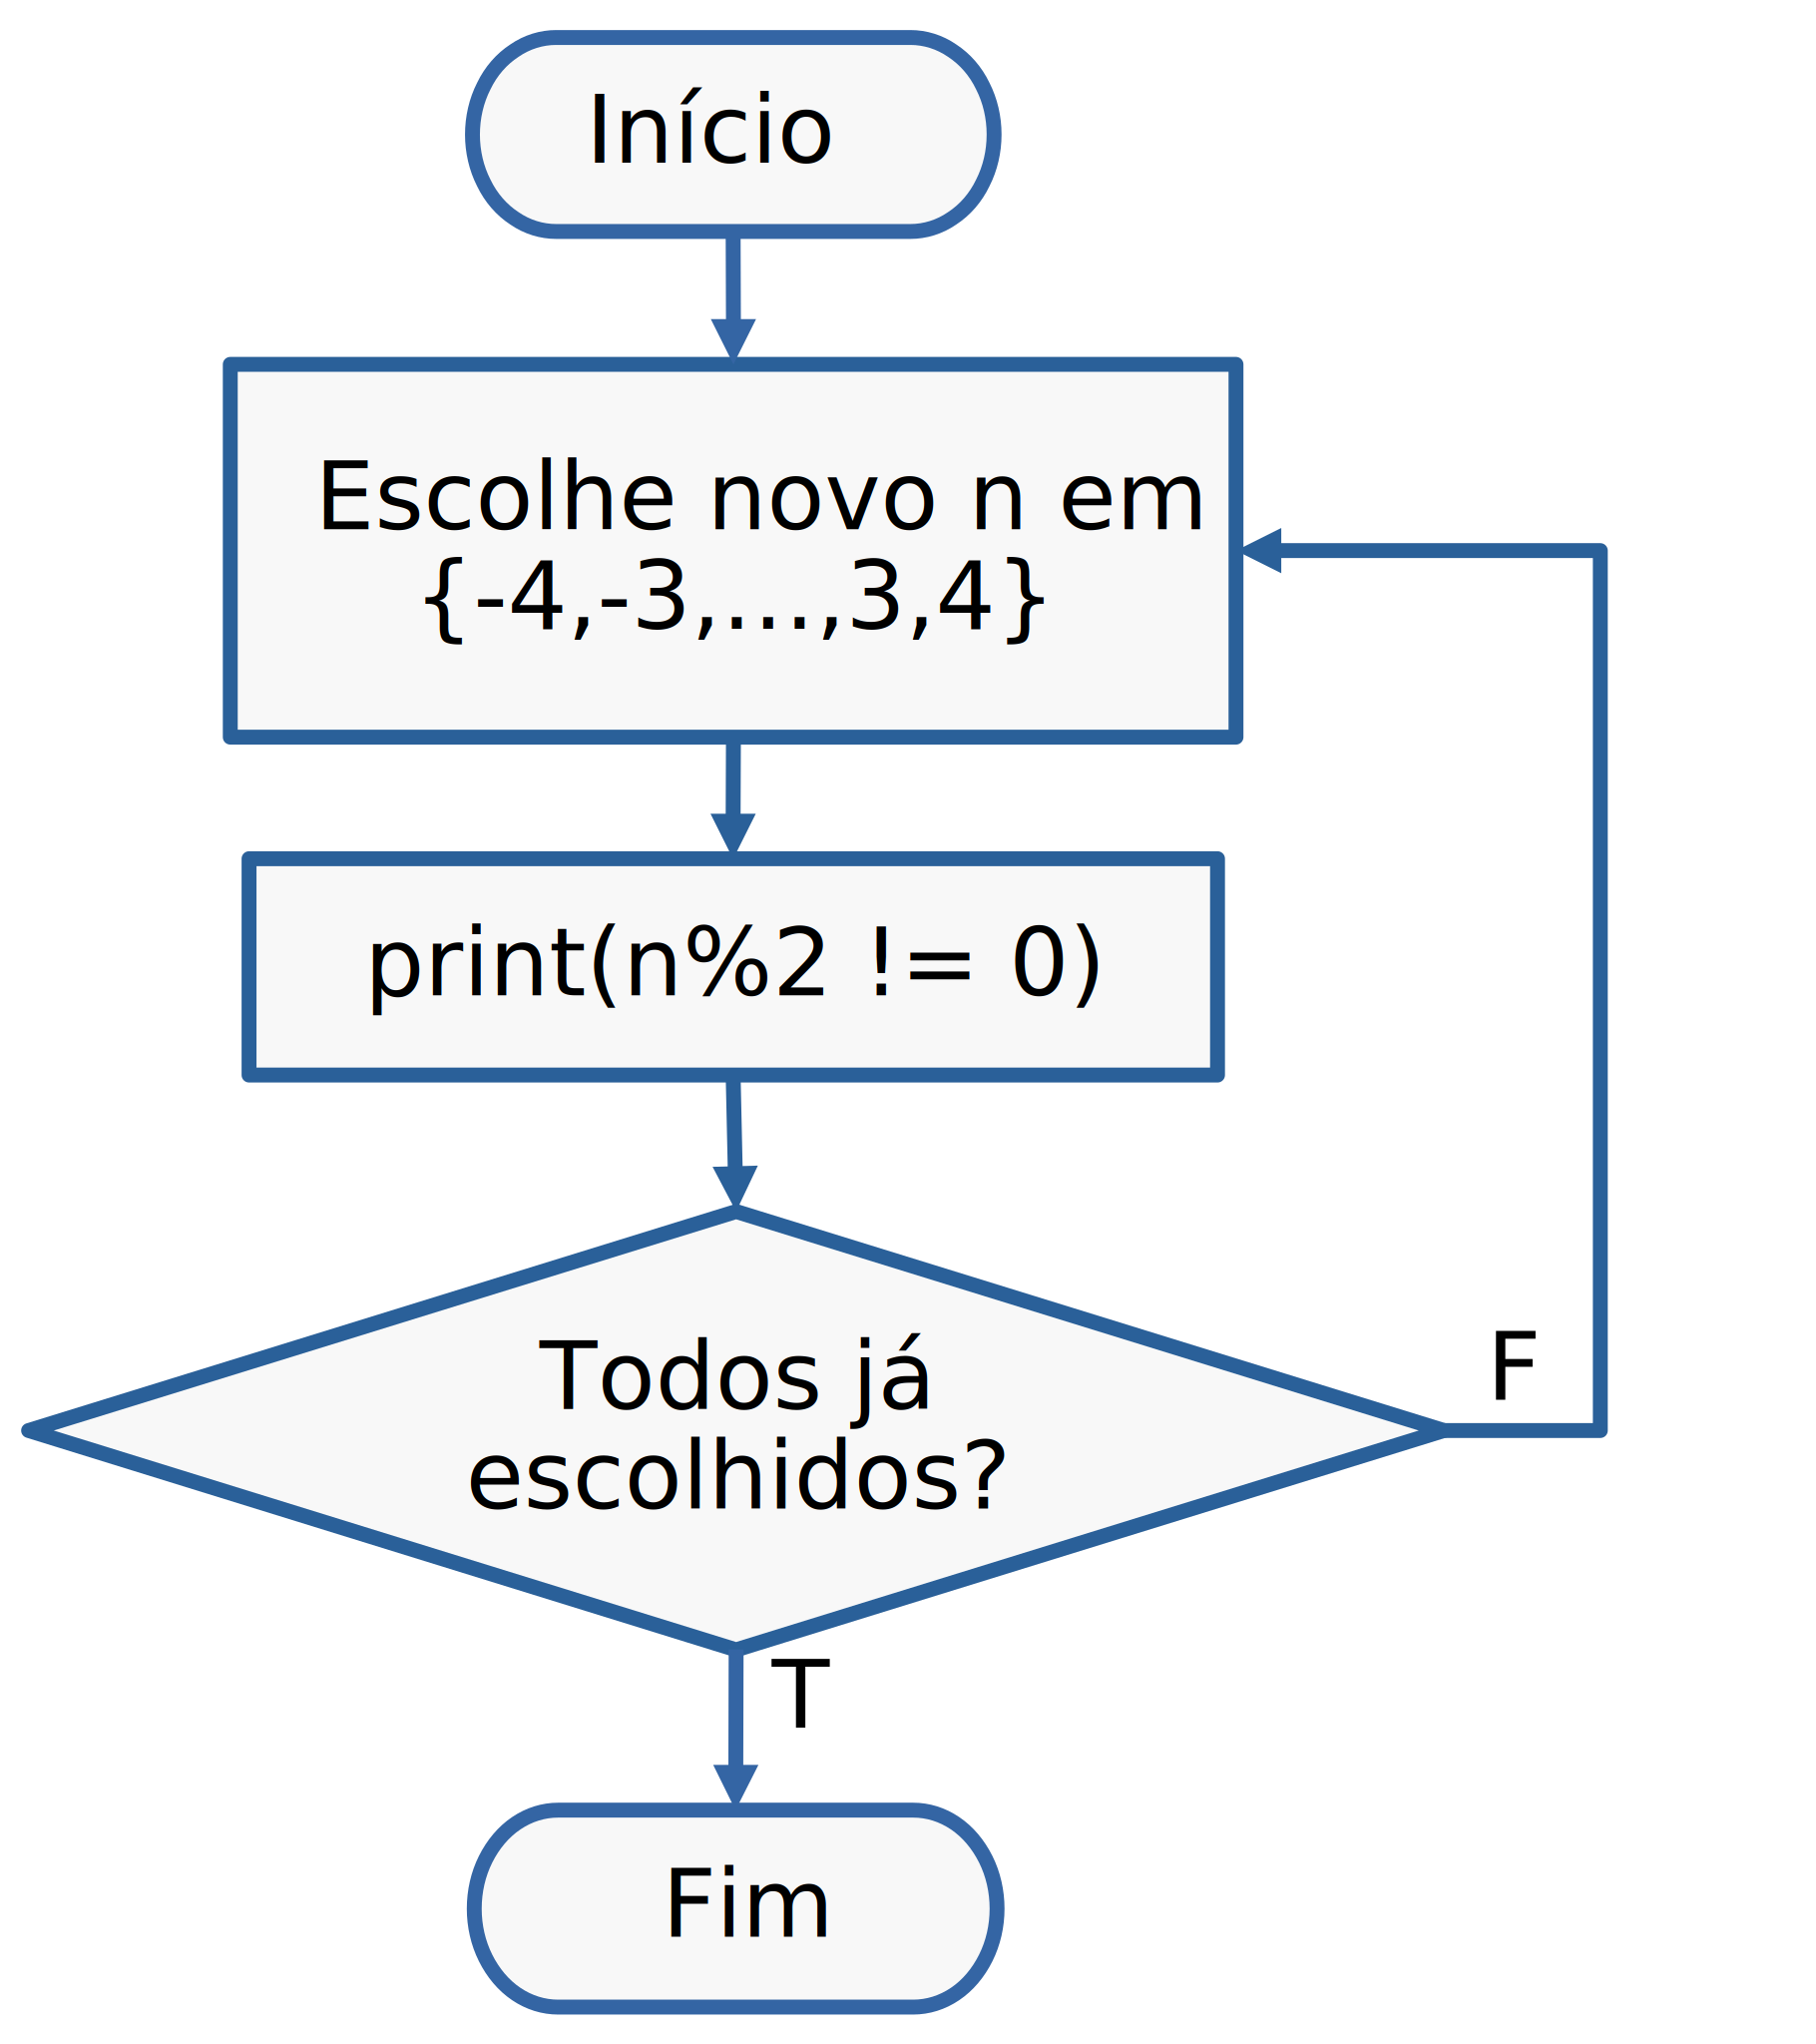
\includegraphics[width=0.4\textwidth]{./cap_fun/dados/fig_leiDosCossenos/fig}
  \end{figure}
  Desenvolva um código que computa e imprime o valor da área de um triangulo de lados $a$, $b$ e $c$ fornecidos por usuária(o).
\end{exer}
\begin{resp}
  Dica: use a \href{https://pt.wikipedia.org/wiki/Lei_dos_cossenos}{lei dos cossenos} e relações fundamentais de triangulo retângulo para obter o valor da altura $h$. 
\end{resp}

\begin{exer}
  Desenvolva um código em que a(o) usuária forneça um ângulo $\theta$ em graus e seja computado e impresso os $\sen(\theta)$ e $\cos(\theta)$.
\end{exer}
\begin{resp}
  Dica: consulte as funções \lstinline+math.sin+, \lstinline+math.cos+.
\end{resp}

\begin{exer}
  Desenvolva um jogo em que a(o) usuária(o) tenha três tentativas para adivinhar um número inteiro entre $0$ a $51$ (incluídos). 
\end{exer}
\begin{resp}
  Dica: O módulo \lstinline+random+ fornece a função \href{https://docs.python.org/3/library/random.html?highlight=random#random.randint}{\lstinline+random.randint(a, b)+} que retorna um inteiro $a \leq x \leq b$.
\end{resp}
